\documentclass[tikz]{standalone}
\usepackage{tikz}
\usetikzlibrary{positioning, graphs}
\usetikzlibrary{graphs.standard}
\begin{document}
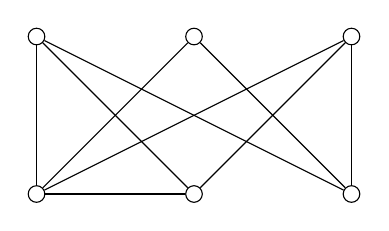
\begin{tikzpicture}
		[mynode/.style={draw,circle,inner sep = 0em, minimum size = 0.6em}]
		\node[mynode] (V 1) at (0,0) {};
		\node[mynode] (V 2) at (2,0) {};
		\node[mynode] (V 3) at (4,0) {};
		\node[mynode] (W 1) at (0,-2) {};
		\node[mynode] (W 2) at (2,-2) {};
		\node[mynode] (W 3) at (4,-2) {};		
		
		\draw (V 1) -- (W 1);
		\draw (V 1) -- (W 2);
		\draw (V 1) -- (W 3);
		\draw (V 2) -- (W 1);
		\draw (V 2) -- (W 3);
		\draw (V 3) -- (W 1);
		\draw (V 3) -- (W 2);
		\draw (V 3) -- (W 3);
		\draw (W 1) -- (W 2);
		

\end{tikzpicture}
\end{document}